\chapter{Problem Statement and Heuristic Solution}
\label{chp:problem_statement}

This chapter describes the details and design considerations of the algorithm presented for solving the problem of optimal mobility management in narrow beam systems. INN Section~\ref{subsec:algo_overview}, examples are given on how to use tables and figures in this MSc thesis.

\section{Scoping the problem}
\label{sec:scope}
\section{User Localization using the optical network}
\label{sec:loc_calc}
\section{Algorithm to optimize mobility management}
\label{sec:algorithm}
Below, we present the algorithm for solving the problem of predictive mobility management. The strategy operates separately for each user, optimizing for maximizing throughput and minimizing latency.
\subsection{High level overview}
Before going in-depth into the algorithm's workings, we present a high-level overview of the handover strategy, specifying the inputs and outputs of the system. Figure~\ref{fig:algo-overview} provides a high-level graphical algorithm overview. Section~\ref{subsec:algo_exp} explains each component in detail in the order of their execution.
\subsubsection{Inputs}
\begin{itemize}
    \item \textbf{User position:} Coordinates of the UE based on the localization method described in Section~\ref{sec:loc_calc}
    \item \textbf{User velocity:} Recorded by the UE as the change in position between two RSRP measurements.
    \item \textbf{Current Serving AP/Beam:} The current optical beam or RF AP serving the UE before the handover procedure is initiated.
    \item \textbf{RSRP report:} An array storing the RSRP measurements recorded by the user for every available serving beam and the RF AP
\end{itemize}
\subsubsection{Outputs}
The algorithm generates a single output:
\begin{itemize}
    \item \textbf{Choice:} the specific AP which the user needs to be switched to to maintain consistent connectivity with the network.
\end{itemize}

\begin{figure}
    \centering
    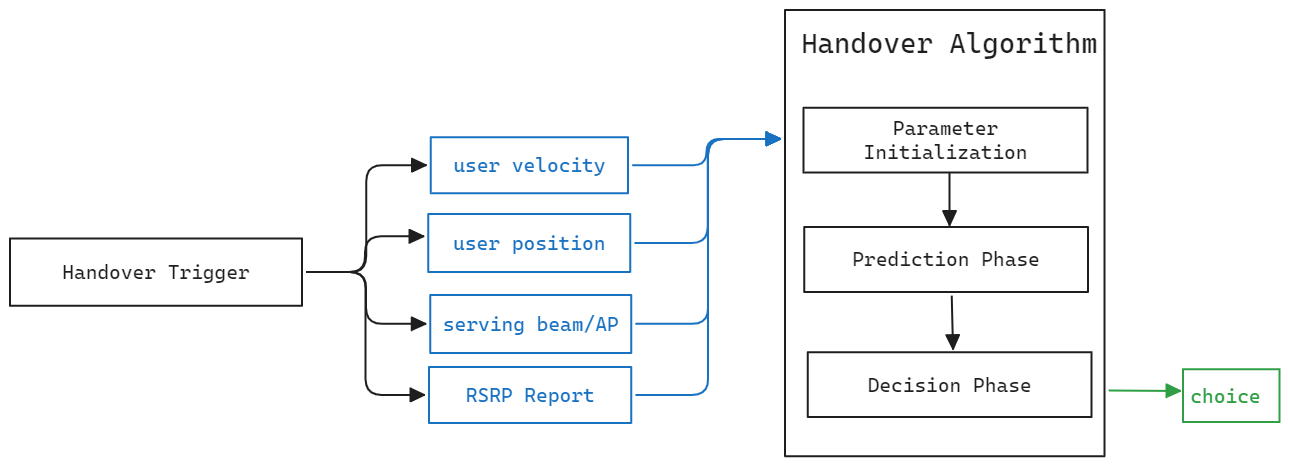
\includegraphics[width=1\linewidth]{Figures/algo-overview.png}
    \caption{High-level overview of algorithm inputs/outputs and components}
    \label{fig:algo-overview}
\end{figure}

% \subsubsection{Sub-components}
% The workings of the algorithm are broadly classified into a pre-process and two consecutive blocks:
% \begin{itemize}
%     \item \textbf{Handover trigger:} Pre-conditions reported by the UE to the network with inputs as described in Subsection~\ref{subsec:algo_overview} which trigger the handover strategy.
%     \item \textbf{Initialization of parameters:} Initialization of meta-parameters dictating the characteristics of a specific instance of the handover decision.
%     \item \textbf{Prediction phase:} The algorithm makes predictions 
%     \item Decision phase
\label{subsec:algo_overview}
\subsection{Detailed explanation}
\label{subsec:algo_exp}
\subsubsection{Handover trigger}
The handover algorithm follows a trigger-based strategy. This means that the handover process is only initiated when specific events or conditions are fulfilled. In this case, the specific trigger for initiating a handover is when RSRP measurements by the UE indicate that another beam/AP is providing a higher SINR. The optical and RF networks periodically send reference signals to the UE, which are then utilized to calculate the RSRP measurements. The reference signals by the optical network also allow for localization information to be tracked. The centers of the 3 beams providing the highest SINR act as the end points for triangulation. Since the reference signal is sent continuously with a set period interval, a change in location between two measurements provides the velocity. The UE reports back the RSRP map as well as the most recent values of position and velocity. When the conditions for the handover are met, the network utilizes the report from the UE as input to initiate the handover strategy. Figure~\ref{fig: handover-trigger} provides a graphical explanation of the handover trigger process.
% 
\begin{figure}
    \centering
    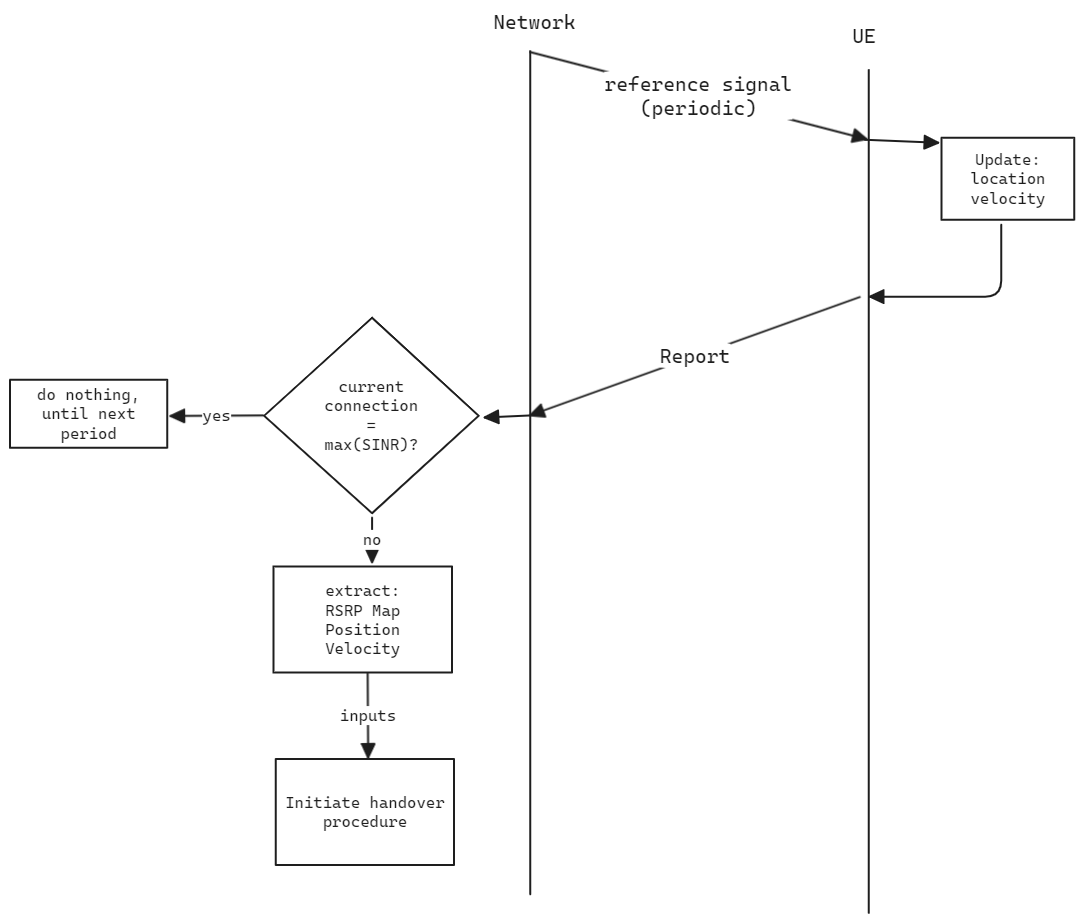
\includegraphics[width=0.75\linewidth]{Figures/handover-trigger.png}
    \caption{Flowchart describing the handover trigger process}
    \label{fig: handover-trigger}
\end{figure}

\subsubsection{Parameter initialization}
We first perform setup for certain parameters characterizing this specific instance of the handover strategy:
\begin{enumerate}
    \item \textbf{Network selection coefficient $\lambda$:} Beyond a certain velocity of the user, it is no longer feasible for the optical network to adequately keep up with the user and provide consistent connectivity. In such situations it is imperative that the algorithm switch the UE to the RF Network. This is mathematically modeled by the network selection coefficient. It is a scaler which indicates the system's preference for the RF network over optical. Higher the velocity of the user, higher is the value of the scaler.
    \item \textbf{Prediction window size $\eta$:} Vertical handovers require more time to perform due to the change in transmission interface. As such, the algorithm must be sure that it would still be most optimal for the user to be connected to the RF network by the time the handover completes. The prediction window size provides a dynamic way of adjusting how far in the future the algorithm will make estimations before making a decision. Vertical Handovers require a larger window size than horizontal handovers. 
    \item \textbf{Prediction step size $t_{TTT}:$} Specifies the time interval between two predictions
    \item \textbf{current time: $t_k:$} Record of the time when the handover process starts, subsequently records the time in the future at which each prediction occurs.
    \item \textbf{current step i:} Starts at 0, specifies how many prediction steps have been taken
    \item \textbf{Score:} Score is an array which keeps track of the SINR measurements throughout the execution of the algorithm. It is analyzed in the decision phase to determine which AP/beam to switch the user to.
    \item \textbf{Decay constant d:} The further we move in the future, The more dependent the estimation becomes on previous predictions. In turn, the probability of the estimation deviating from ground reality increases. To compensate for such a potential error, We utilize exponential decay on the score per timeslot. Thus, as the predictions move further in the future, their impact on the score and thus the final decision reduces as well.
\end{enumerate}

\subsection{Prediction phase}
As long as we have not iterated through the entire prediction window $(i < \eta)$, for each step we do the following:
\begin{enumerate}
    \item Predict the location at the next time step. The short term prediction is given by (~\ref{eq:pred-loc})
    \begin{equation}
        p(t_k + t_{TTT}) \leftarrow p(t_k) + v(t_k) \times t_{TTT} + \frac{1}{2}a{t_k} \times t_{TTT}^2
        \label{eq:pred-loc}
    \end{equation}
    \item Based on the predicted location we make an estimate of the SINR from each beam/AP. The SINR from the RF AP is scaled by the network selection coefficient as explained in Parameter initialization. These are utilized as the score for that AP/beam in this slot.
    \item The score array is updated with the new values from this time slot after scaling them by the decay factor.
\end{enumerate}
Figure~\ref{fig:algo-prediction} showcases the operations that take place in each time-slot of the prediction window.
\begin{figure}
    \centering
    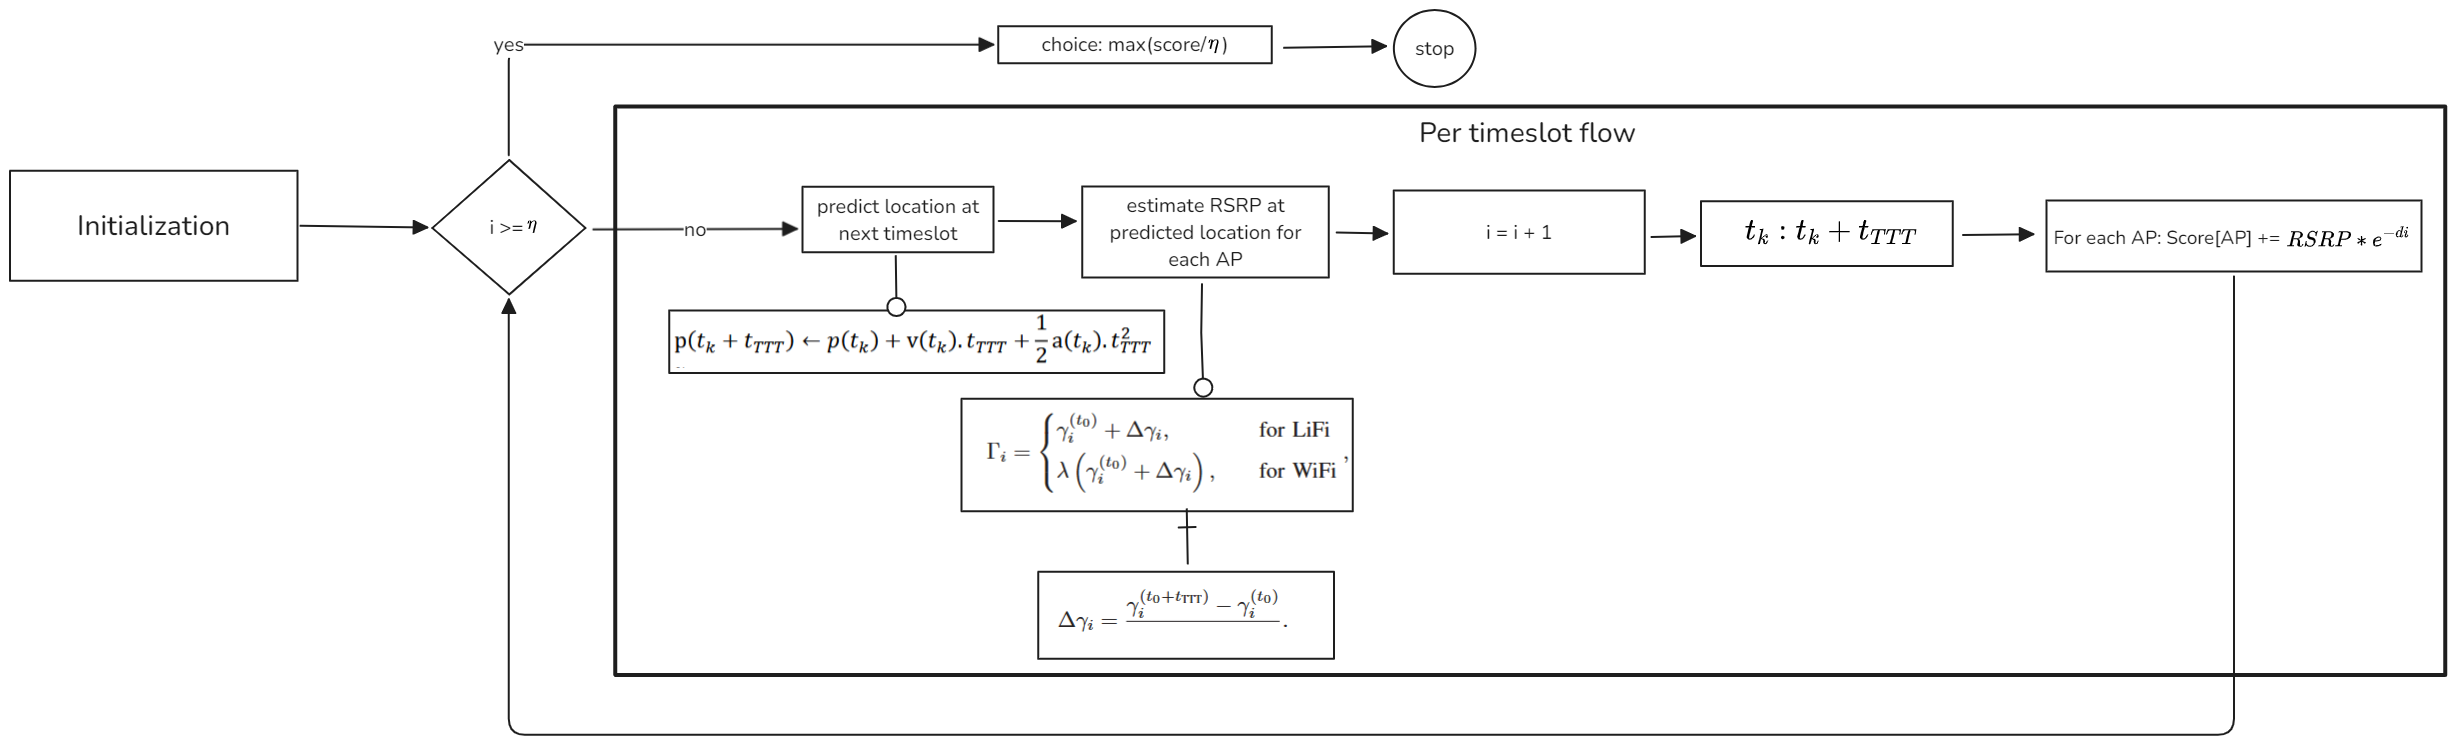
\includegraphics[width=1\linewidth]{Figures/algorithm-prediction-phase.png}
    \caption{Prediction phase of the algorithm: showcasing operations conducted each time-slot}
    \label{fig:algo-prediction}
\end{figure}
\subsection{Decision phase}
Once the prediction phase has been carried out for each slot in the prediction window, the algorithm makes a decision on which AP to connect the user to. The algorithm selects the AP with the greatest average score as given by ().
\begin{equation}
        {choice} = \max(\frac{score}{\eta})
        \label{eq:algo-decide}
    \end{equation}
% Define models with math, such that
% %
% \begin{equation}
% x = a^2 + b^2,
% \label{eq:EQUATION}
% \end{equation}
% %
% where $a$ and $b$ are your parameters, define your system.

% Remarks on style:

% \begin{enumerate}
% 	\item use `Section` name to refer to sections when citing (so Section~\ref{sec:SECTIONTITLE} not Sec.~\ref{sec:SECTIONTITLE} or Subsection~\ref{sec:SECTIONTITLE}); Same comment applies to Tables, Algorithms and Figures
% 	\item Tables and figures must be at the top of the page---use [t] marker (not [h], for `here`); 
% 	\item Every caption should end with a period;
% 	\item Encapsulate equations in `()` brackets and do not add word `equation before` (therefore `in~(\ref{eq:EQUATION})`, not `in Equation~\ref{eq:EQUATION}` or in Eq.~\ref{eq:EQUATION});
% 	\item Equations are sentences, so punctuation applies at the end of it (comma, semicolon or full-stop).
% \end{enumerate}

% Here is a simple table

% \begin{table}[t]
% \centering
% \begin{tabular}{| l | c | r |}
% \hline
% left aligned & centred & right aligned \\
% \hline \hline
% 12 & 34 & 56 \\
% \hline
% \end{tabular}
% \caption{Complete sentence describing the tabular data. Caption should summarize the conclusions of the result.}
% \label{tab:table_1}
% \end{table}

% Here is a simple figure.

% \begin{figure}[t]
% \includegraphics[width=\textwidth]{template-pics/tud-es-logo-tikz/tud-es-logo}
% \caption{Complete sentence describing the figure thoroughly. Caption should summarize the conclusions of the result.}
% \label{fig:example-figure}
% \end{figure}

% Citations are here~\cite{polastre2004analysis,powercast_website,hester2016persistent,schaper_msc_thesis_2017,dementyev_uist_2016}. See `bib/MyMScTUDESThesisBibFile.bib` file for a list of requirements when typesetting a bibliography.
